In this paper, we propose a robust defence system called \textit{Apollon}, which is designed to protect an IDS against AML
attacks.
\textit{Apollon} is composed of multiple layers to provide better security than traditional IDS and previous works that rely
solely on training with adversarial traffic.
The proposed system combines multiple classifiers, a \textit{Multi-Armed Bandits (MAB)} algorithm, and requests clustering to
provide robust defence against AML attacks.

\begin{figure*}
    \centering
    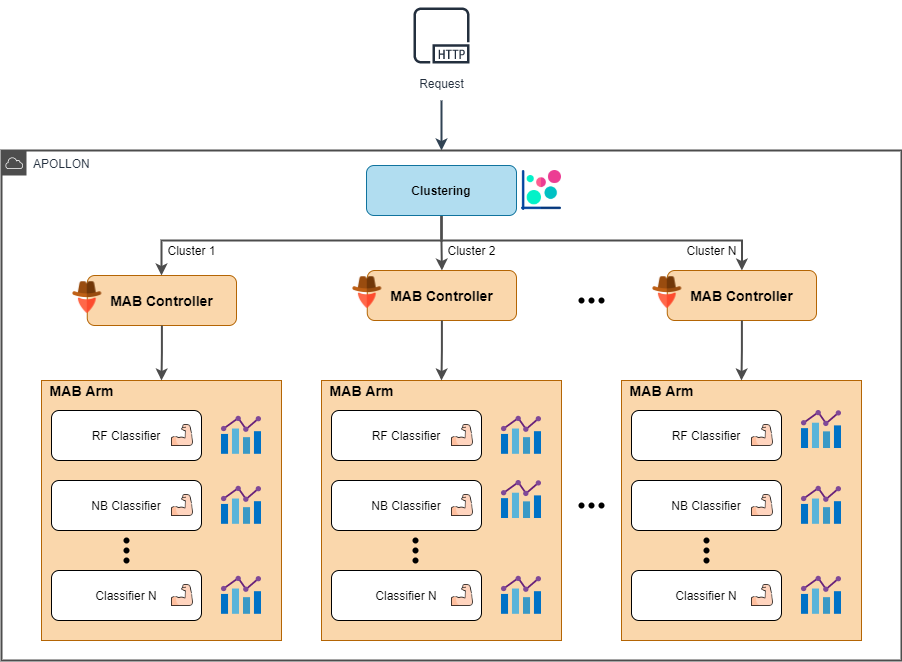
\includegraphics[width=0.9\textwidth]{Apollon.png}
    \caption{\textit{Apollon} Architecture}
    \label{fig:apollon-architecture}
\end{figure*}


The first layer of Apollon involves using multiple classifiers instead of a single classifier that is traditionally
used in IDS.
The concept behind utilizing multiple classifiers is to increase the difficulty for potential attackers attempting to
replicate the IDS model.
This is because they cannot predict which specific model will be responsible for classifying a given request.

To dynamically select the optimal classifier or set of classifiers for each input, \textit{Apollon} involves using
a \textit{Multi-Armed Bandits (MAB)} with \textit{Thompson sampling}.
The \textit{MAB} is responsible for selecting the arm (classifier) to use for each request based on the current state of the
system.

Finally, requests are clustered, and there is a version of each classifier for each cluster, trained only with the
information of that cluster.
Clustering is used to add another layer of uncertainty to the system, as the attacker cannot predict in a simple way which
cluster a request belongs to.

With \textit{Apollon}, we are able to maintain the performance of traditional IDSs when it comes to network traffic without
AML attacks.
We achieve this by utilizing the best classifiers for each type of request.
Additionally, \textit{Apollon} offers a solution to prevent attackers from easily learning from the behavior of our classifiers
through AML techniques.

Figure~\ref{fig:apollon-architecture} shows the architecture of \textit{Apollon}, and the flow that a network traffic request
follows until it is classified.

Listing~\ref{lst:apollon-training-process} shows the output of an Apollon training process example with two clusters and three
classifiers.
As can be seen, the training data is first divided between the two clusters, the classifiers are trained for each cluster and
finally, the rewards are assigned.
The Listing~\ref{lst:apollon-classifier-selection-process} shows a selection process example of the classifier for each request,
the predicted value and the real value.

\begin{lstlisting}[caption={Apollon training process example}, label={lst:apollon-training-process}, frame=single, captionpos=b, basicstyle=\fontsize{9}{11}\selectfont\ttfamily]
    Cluster 0: Len of request 274888
    Training arm 0 on cluster 0
    Training arm 1 on cluster 0
    Training arm 2 on cluster 0
    Cluster 1: Len of request 358525
    Training arm 0 on cluster 1
    Training arm 1 on cluster 1
    Training arm 2 on cluster 1

    Setting reward_sums arm 0 on cluster 0
    Setting reward_sums arm 1 on cluster 0
    Setting reward_sums arm 2 on cluster 0
    Setting reward_sums arm 0 on cluster 1
    Setting reward_sums arm 1 on cluster 1
    Setting reward_sums arm 2 on cluster 1
\end{lstlisting}

\begin{lstlisting}[caption={Apollon classifier selection process example}, label={lst:apollon-classifier-selection-process}, frame=single, captionpos=b, basicstyle=\fontsize{9}{11}\selectfont\ttfamily]
    Selected arm: 0.0    Predicted:0    Actual:0
    Selected arm: 0.0    Predicted:0    Actual:0
    Selected arm: 2.0    Predicted:0    Actual:0
    Selected arm: 0.0    Predicted:0    Actual:0
    Selected arm: 1.0    Predicted:1    Actual:1
    Selected arm: 2.0    Predicted:0    Actual:0
\end{lstlisting}

In the following, each of the layers that influence the final classification of a network traffic request will be
detailed.


\subsection{Multiple Classifiers}\label{subsec:multiple-classifiers}
The first layer of \textit{Apollon} involves using multiple classifiers instead of a single classifier, which is typically used
in traditional IDS.
The idea of using multiple classifiers is to make it more difficult for the attacker to replicate the IDS model,
as he is not able to predict which model is going to classify the request.
By utilizing a greater number of diverse classifiers, the system becomes more resilient by introducing greater uncertainty,
and better classifiers implies better performance in the \textit{Apollon} system score.

In \textit{Apollon}, we can use any type of classifier.
These classifiers can be either the most common ones based on Deep Learning or Machine Learning, or classifiers based
on network traffic request forecasting techniques, or the more classical ones based on rule systems.

\subsection{Multi-Armed Bandit}\label{subsec:multi-armed-bandit}
The second layer of the \textit{Apollon} defence system involves the use of a \textit{Multi-Armed Bandits (MAB)} algorithm
to select the appropriate classifier or set of classifiers for each network traffic request.
The \textit{MAB} is responsible for selecting the best classifier or set of classifiers to evaluate whether a request is benign
or malicious.
This approach avoids the need for manual tuning of thresholds or weights for each classifier.

The \textit{MAB} algorithm works by selecting the arm, or classifier, that has the highest probability of providing the correct
classification.
In \textit{Apollon}, we use \textit{Thomson Sampling}, which is a popular algorithm for solving the \textit{MAB} problem.
Thomson Sampling balances exploration and exploitation of the available classifiers, ensuring that the system selects
the optimal classifier or set of classifiers while still being responsive to new and unknown types of traffic.

The \textit{MAB} algorithm in \textit{Apollon} is designed to take into account the different types of classifiers used in the system.
For instance, if the \textit{Random Forest} classifier has a high probability of being correct, but the \textit{Naive Bayes} and
\textit{Logistic Regression} classifiers have lower probabilities, the \textit{MAB} algorithm will select the \textit{Random Forest}
classifier for that particular request.
In this way, the \textit{MAB} algorithm ensures that the system selects the optimal set of classifiers for each request,
improving the overall accuracy of the classification.

The \textit{MAB} algorithm is constantly updating the probabilities of the different classifiers based on their previous
performance.
Thus, the system can adapt to changes in the traffic patterns over time, ensuring that the system is always up to date
with the latest types of attacks.
This update process is described in Algorithm \ref{alg:thompson-sampling}.
Here, $S_i$ and $F_i$ are the number of observed successes and failures for arm $i$, respectively, and $theta_i$ 
is the estimated probability of obtaining a positive reward from arm $i$.
The algorithm uses the Beta distribution as an a priori distribution for the parameters $theta_i$, and updates it
with the observed data using Bayes' theorem.
The algorithm chooses the arm (ML classifier) that has the highest probability of being the best according to the
samples from the posterior distribution.

\begin{algorithm} 
    \caption{\textit{Apollon} Thompson Sampling}
    \label{alg:thompson-sampling}
    \begin{algorithmic}
        \State Intit $S_i = 0$ y $F_i = 0$ for each arm $i$
        \For{$t = 1, 2, \dots$}
            \State For each arm $i$, sample $\theta_i$ of Beta distribution ($S_i + 1$, $F_i + 1$)
            \State Choose the arm $I_t$ that maximizes $\theta_i$
            \State Observe the reward $X_t$ of the arm $I_t$.
            \If{$X_t = 1$}
                \State Increment $S_{I_t}$ by one
            \Else
                \State Increment $F_{I_t}$ by one
            \EndIf
        \EndFor 
    \end{algorithmic} 
\end{algorithm}

By using a \textit{Multi-Armed Bandits} algorithm, \textit{Apollon} can dynamically select the optimal classifier or set of classifiers
for each network traffic request, making the system more responsive to new types of attacks.
The use of \textit{Thomson Sampling} ensures that the system is balanced between exploration and exploitation, improving the
overall attacks detection rate of the classification.
Figure~\ref{fig:mab-algorithm} shows the diagram of the \textit{MAB} algorithm with multiple classifiers.

\begin{figure}
    \centering
    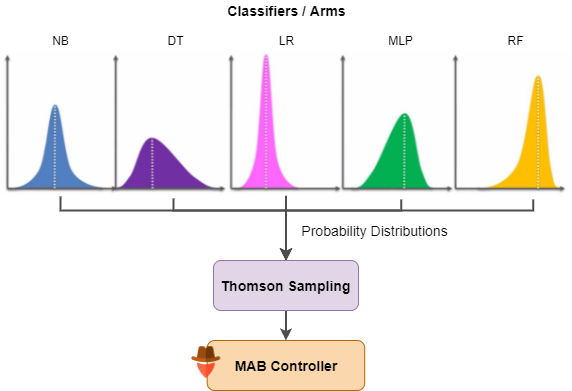
\includegraphics[width=0.9\columnwidth]{ApollonMAB.png}
    \caption{Apollon \textit{Multi-Armed Bandits} algorithm with multiple classifiers}
    \label{fig:mab-algorithm}
\end{figure}


\subsection{Traffic requests clustering}\label{subsec:traffic-requests-clustering}
The final layer of the \textit{Apollon} defence system involves clustering the network traffic requests based on their
features, and then training a separate version of each classifier for each cluster.
By doing this, the system is able to achieve higher accuracy for each cluster by training the classifiers specifically
for the traffic patterns in that cluster.

The traffic requests are clustered using the \textit{K-Means} algorithm~\cite{sinaga2020unsupervised}, which is a
popular clustering algorithm that is used in many Machine Learning applications.
The \textit{K-Means} algorithm works by randomly selecting $k$ points as the initial centroids, and then iteratively
updating the centroids until the clusters converge.
In \textit{Apollon}, we use the \textit{K-Means} algorithm to cluster the network traffic requests based on their features,
ensuring that requests with similar features are grouped together.
These features are the same ones used by the classifiers to evaluate the requests, ensuring that the clustering is
based on the same information that the classifiers use to make their decisions.

For each cluster, a separate version of each classifier is trained using only the traffic requests in that cluster.
This ensures that each classifier is specifically tuned to the traffic patterns in that cluster.

When a new network traffic request arrives at \textit{Apollon}, it is classified into the appropriate cluster based on
its features.
The \textit{Multi-Armed Bandits} algorithm is then used to select the optimal set of classifiers for that cluster,
taking into account the performance of each classifier in that specific cluster.
Then, the selected classifier or set of classifiers evaluate the request and determine whether it is benign or malicious.

By clustering the network traffic requests and training separate versions of each classifier for each cluster,
\textit{Apollon} allows the \textit{Multi-Armed Bandit} algorithm to generate multiple probability distributions for
each classifier, depending on the type of request received.
This combination of techniques makes it challenging for potential attackers to identify the classifier providing the
response, reducing the likelihood of successful imitation.